\documentclass{article}
\usepackage{graphicx}
\usepackage{float}
\usepackage[spanish]{babel}
\usepackage{hyperref}
\usepackage{csquotes}
\graphicspath{ {img/} }
\setlength{\parskip}{\baselineskip}

\title{Diseño de Base de la Datos \\[3ex] \small PAMN - Programación de Aplicaciónes Moviles Nativas}

\author{Chamil José Cruz Razeq}

\begin{document}
    \maketitle
    \thispagestyle{empty}
    \newpage

    \section{Introducción}
        Todas las tareas propuestas se encuentran disponibles en el siguiente
         repositorio de \href{https://github.com/chamilstudy/ulpgc_pamn_assigments}{GitHub}.

    \section{Identificación de la capa de persistencia}
    Para el desarrollo de la aplicación planteada en el \cite[Lab 3]{lab3} se planteó aplicar
     el modelo MVVM [Figura \ref{fig:mvvmdiagram}], identificando los siguiente elementos:
    
    \begin{itemize}
        \item VistaAreas, ModeloVistaAreas y ModeloAreas: con información reducida
               de cada area [Figura \ref{fig:areasdiagram}].
        \item VistaAreaEspecifica, ModeloVistaAreaExpecifica y ModeloAreaEspecifica:
               con información detallada de un área especificada.
        \item VistaSOS, ModeloVistaSOS y ModeloSOS: con información de los medios de
               seguridad y emergencias.
        \item VistaSolicitud, ModeloVistaSolicitud y ModeloSolicitud: gestionando el
               formulario de solicitudes de uso de áreas recreativas.
        \item VistaSolicitudes, ModeloVistaSolicitudes y ModeloSolicitudes: gestionando
               las solicitudes de uso de áreas recreativas.
    \end{itemize}

    \begin{figure}[H]
        \centerline{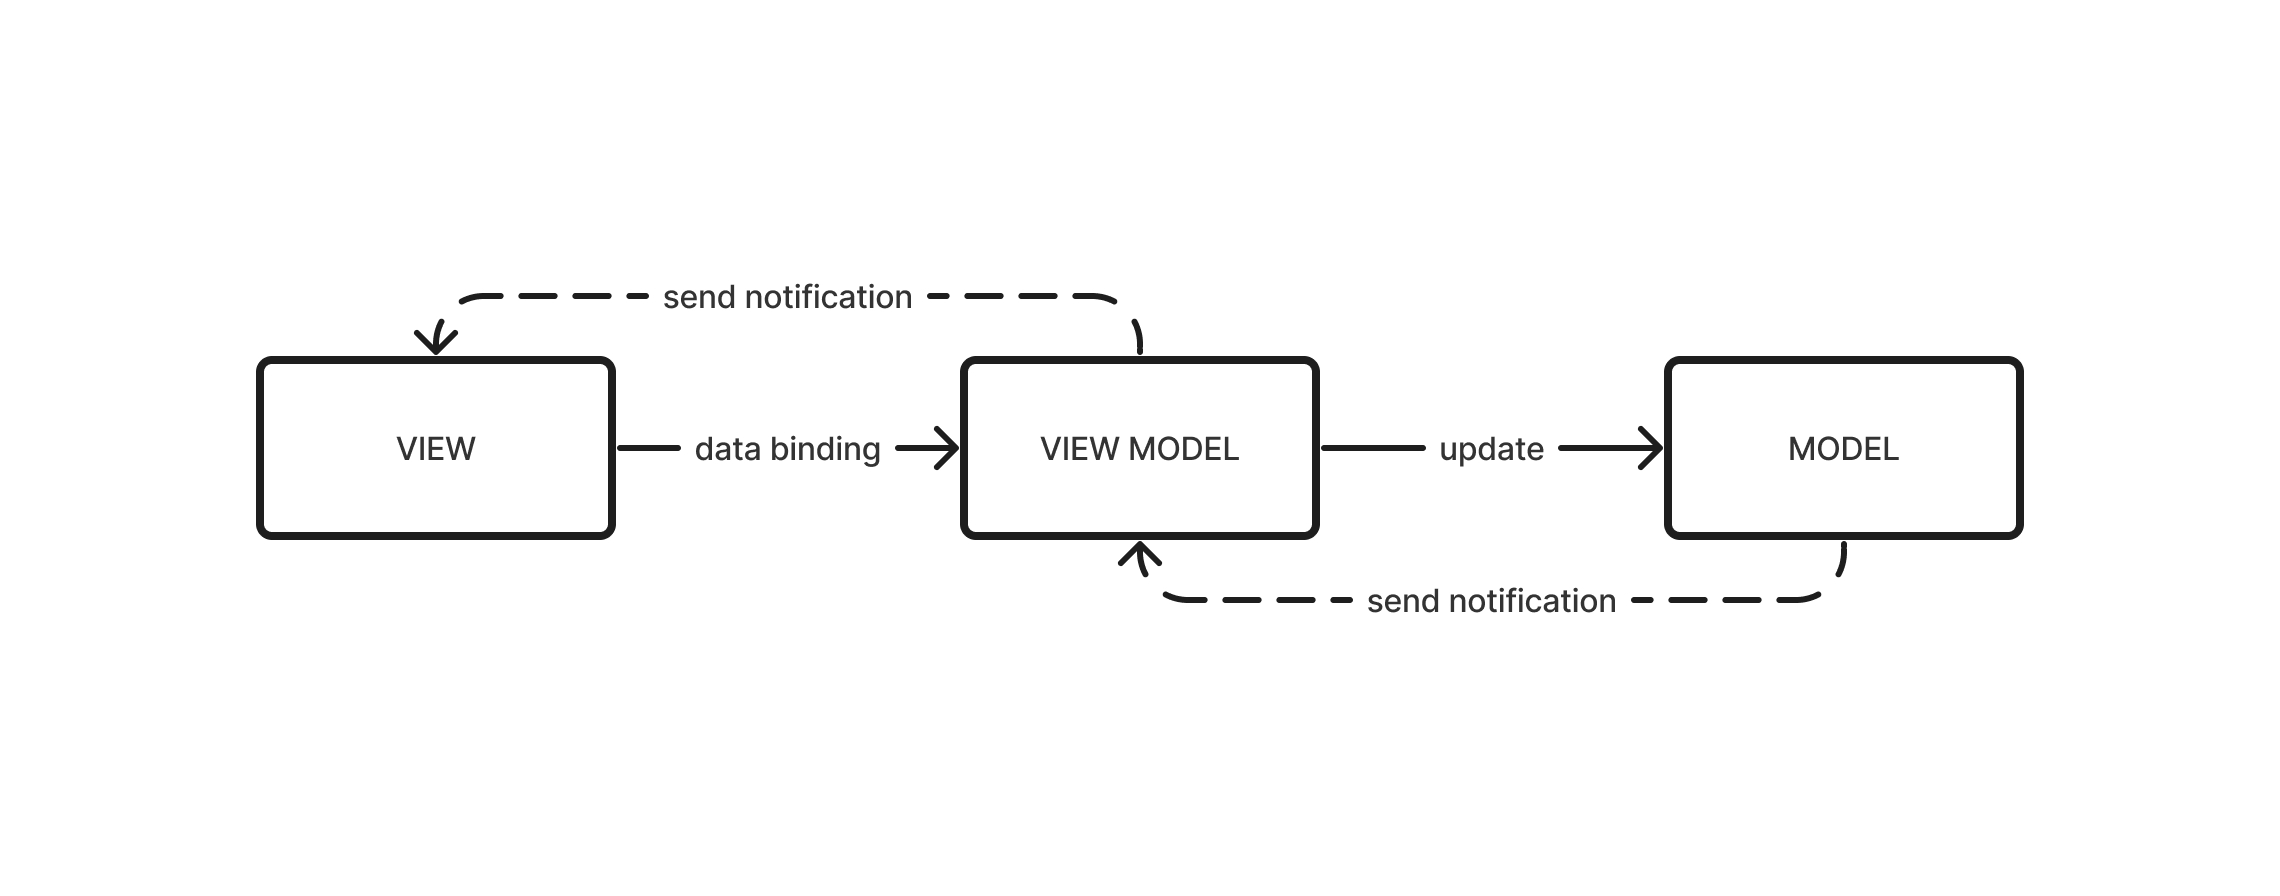
\includegraphics[scale=0.4]{mvvmdiagram}}
        \caption{Diagrama de MVVM}
        \label{fig:mvvmdiagram}
    \end{figure}

    \begin{figure}[H]
        \centerline{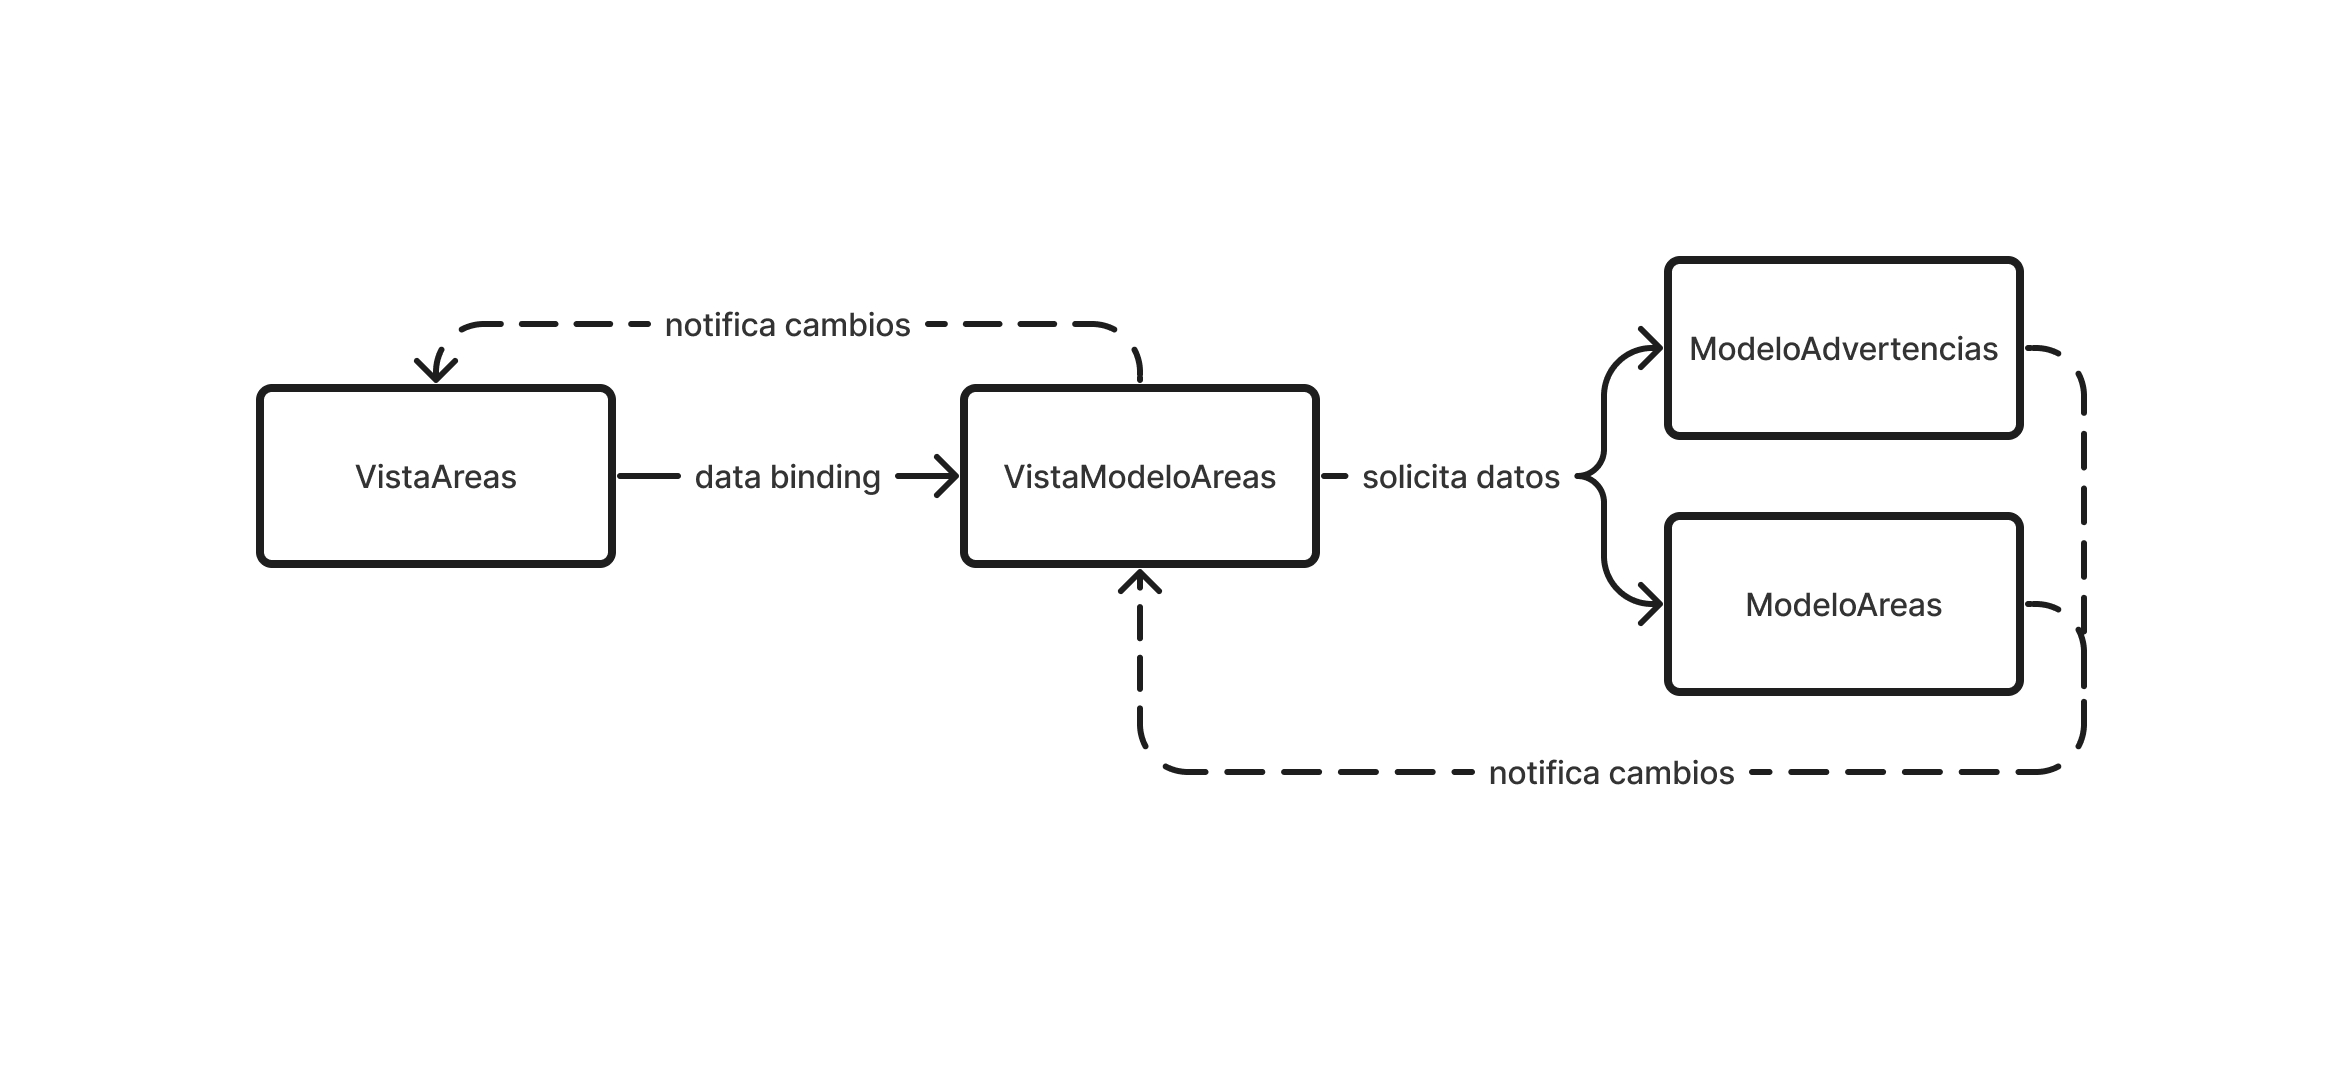
\includegraphics[scale=0.4]{areasdiagram}}
        \caption{Diagrama de MVVM}
        \label{fig:areasdiagram}
    \end{figure}
    
    Donde encontramos los modelos relacionados con la persistencia de datos:

    \begin{itemize}
        \item ModeloAreas: conjunto de ModeloAreaEspecifica.
        \item ModeloAreaEspecifica: información sobre un area.
        \item ModeloSOS: información de los medios de seguridad y emergencias.
        \item ModeloSolicitudes: información sobre las solicitudes.
    \end{itemize}
    
        
    \section{Selección de tecnología}
    De los modelos anteriores hemos identificado que algunos constituirán
     información que deberá ser actualizada en tiempo real, y otros que conformarán
     datos de carácter especifico que no sufrirá cambios, al menos en corto plazo.
     Por este motivo se ha decidido utilizar \enquote*{Rooms} para la capa local; por
     su flexibilidad y rapidez, además de gran documentación y aceptación en el
     desarrollo en android; y \enquote*{Firebase} para la capa externa; por su fiabilidad
     y facilidad de aplicación.
    
    \section{Definición de un Modelo}
    Continuando con el apartado anterior, se ha tomado como referencia los modelos De
     advertencias y areas, respectivamente. Como podemos observar en la imagen
     [Figura \ref{fig:bbdddiagram}], para uno de los modelos se tiene en cuenta el uso
     de una API para solicitar la información a la base de datos alojada en Firebase,
     mientras que en el otro modelo se hace uso de la arquitectura de \enquote*{Rooms},
     definiendo una entidad y un \enquote*{DAO} que se comunica con la base de datos en
     \enquote*{SQLite}.

    \begin{figure}[H]
        \centerline{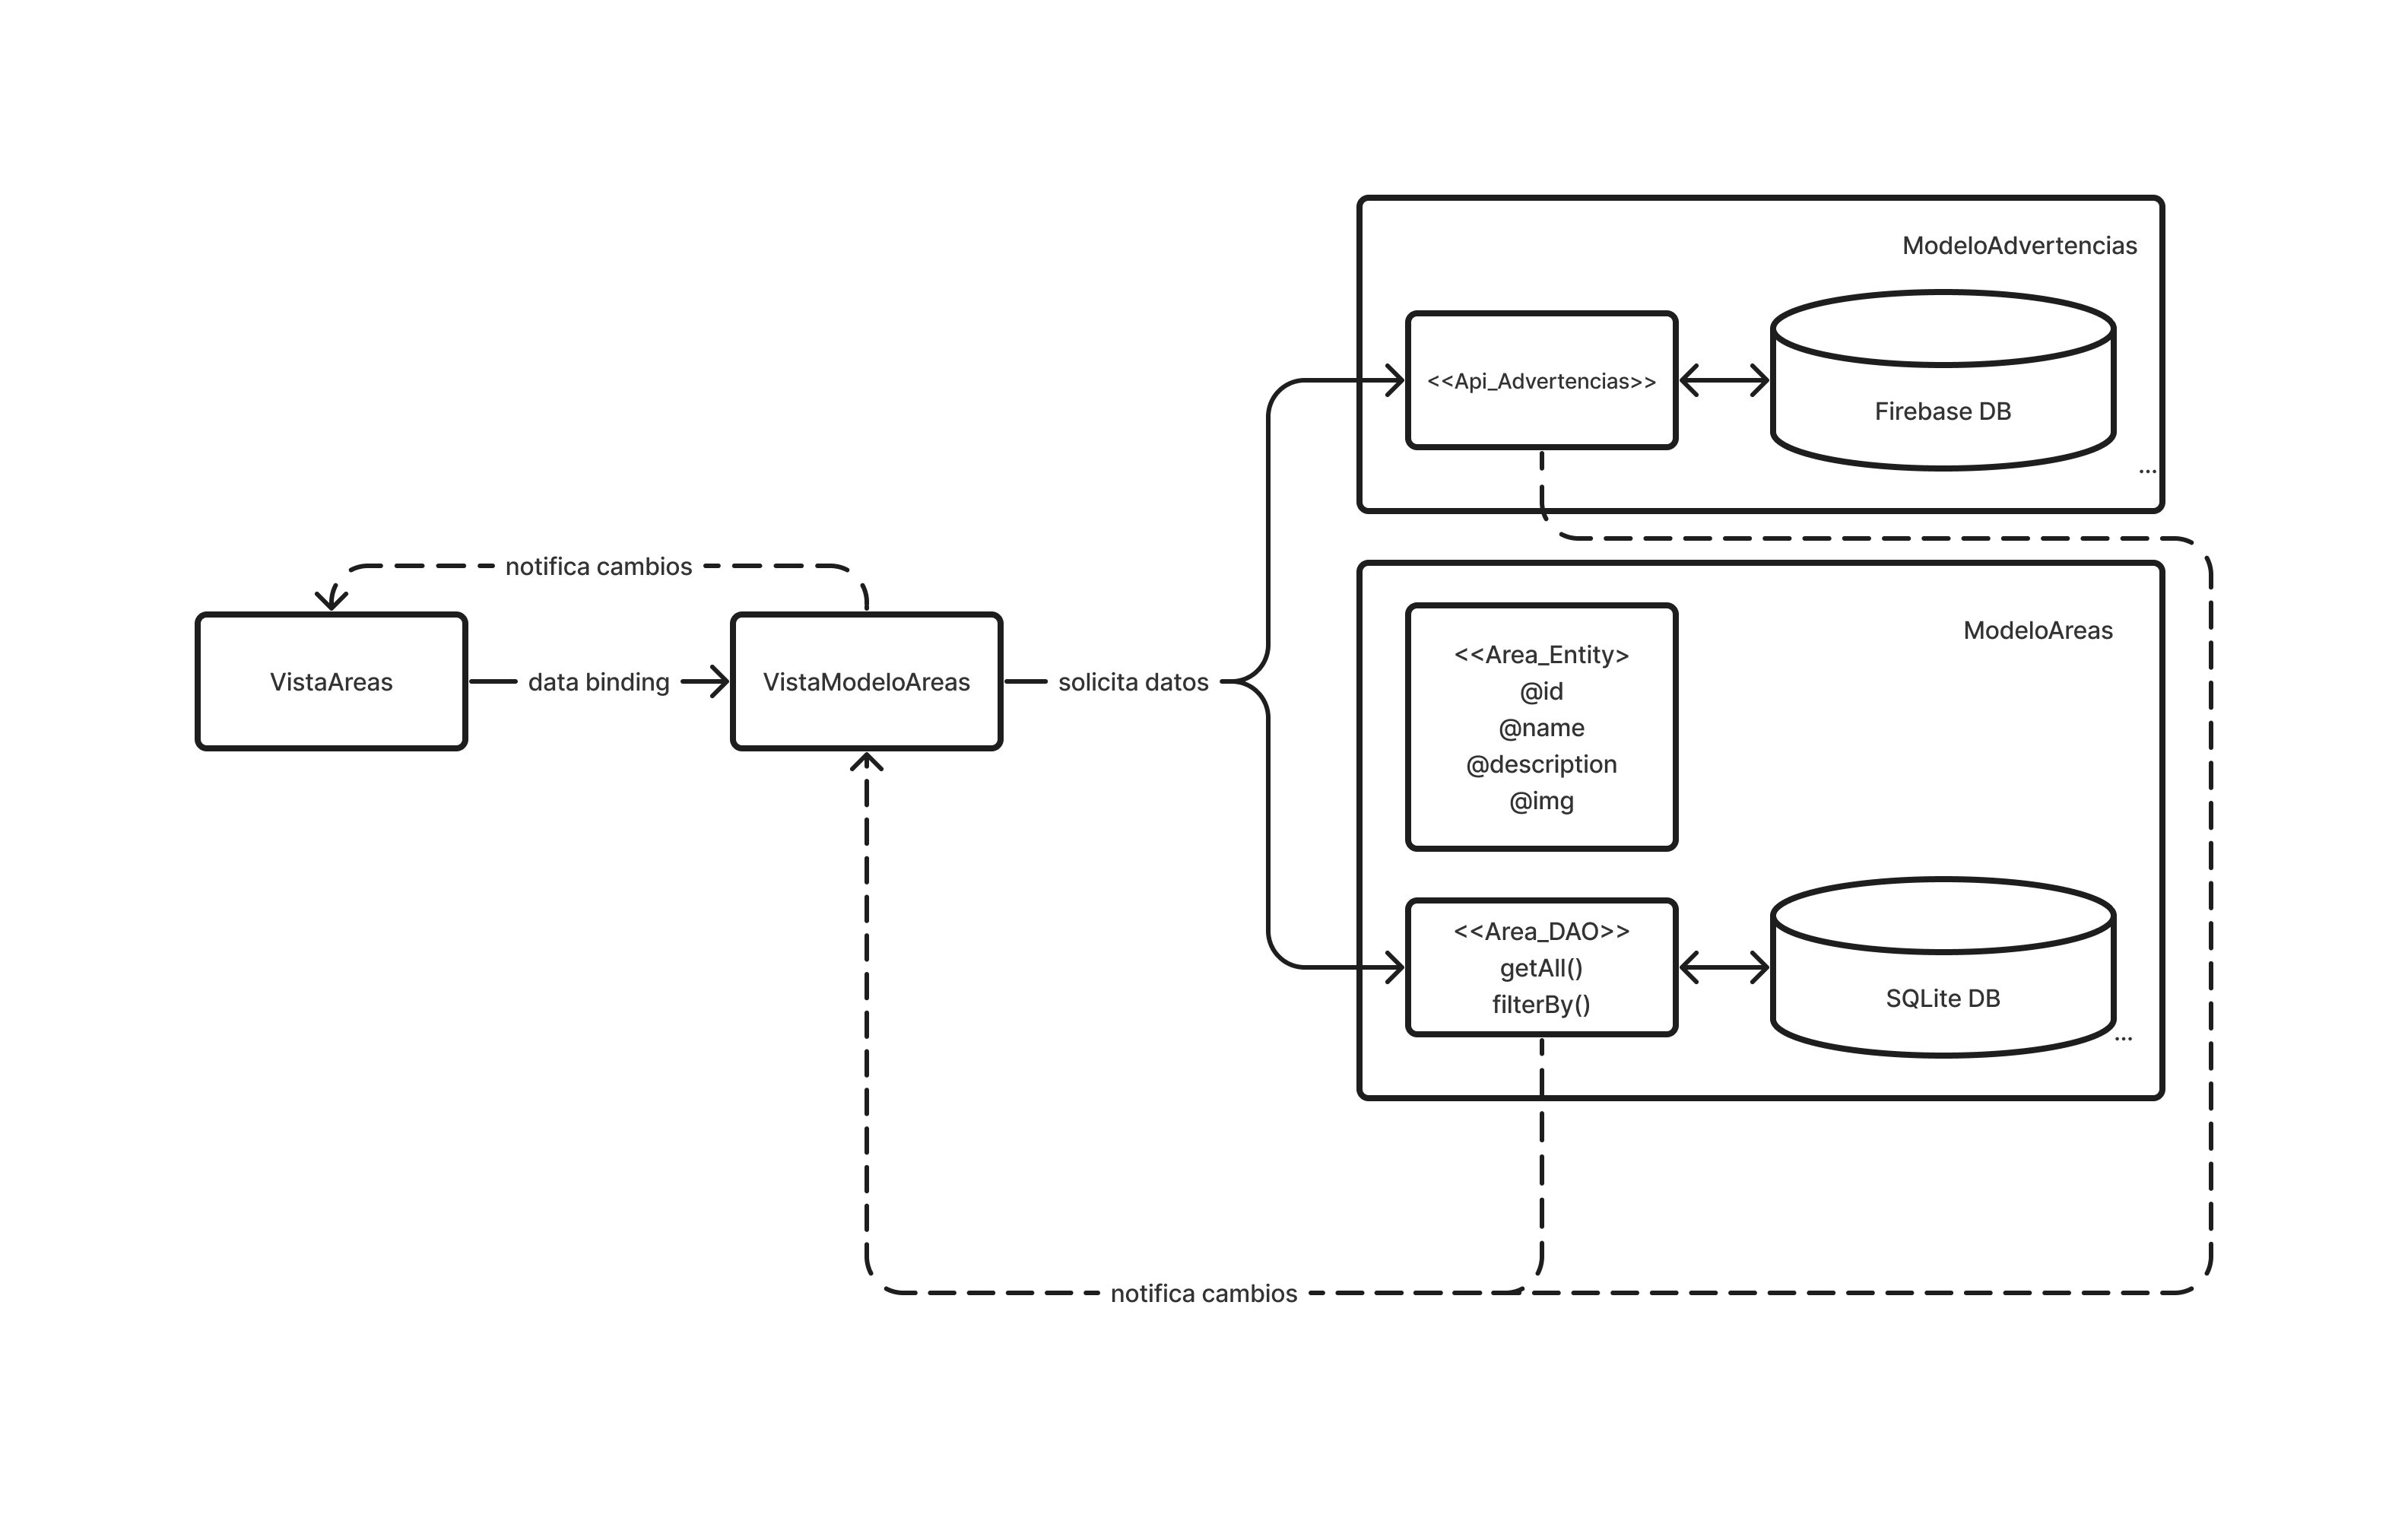
\includegraphics[scale=0.3]{bbdddiagram}}
        \caption{Diagrama de MVVM}
        \label{fig:bbdddiagram}
    \end{figure}

    \section{Conclusión}
    Finalmente, respondiendo a las preguntas formuladas en el enunciado de la actividad.
    
    \begin{itemize}
        \item ¿Qué pasa si en un futuro se quisiera cambiar el motor de base de datos?
        Localmente una migración sería parcialmente sencilla ya que \enquote*{Rooms}
         actúa como una especie de puente con \enquote*{SQLite}, por lo que podría migrarse
         a otra estructura similar con cierta facilidad. Respecto a \enquote*{Firebase}, utilizamos
         una \enquote*{API}, lo cual podría facilitar el uso de otros servicios, pero con el matiz
         de tener que realizar una migración desde un servicio a otro, con los costes que ello
         implica, en caso de que ambas plataformas lo permitan con cierta facilidad.
        \item ¿Qué partes de tu aplicación tendrías que modificar?
        En el caso local, dependiendo de la nueva tecnología, sustituir las \enquote*{entidades} y
         \enquote*{DAO} por sus equivalentes. Por otro lado con \enquote*{Firebase}, dependiendo
         del servicio destino, que herramientas facilitan para la migración, y los ajustes
         oportunos que sean necesarios en cuanto a la \enquote*{API}.
        \item ¿Qué dificultades anticipas?
        La posible curva de aprendizaje con las nuevas tecnologías a usar, las nuevas estructuras a
         desarrollar y la migración de los datos persé (en caso de poderse realizar).
        \item ¿Cómo podrías diseñar tu aplicación para minimizar el impacto de tal cambio?
        Reduciendo la variedad de servicios a utilizar, y utilizando tecnologías que posean herramientas
         que faciliten la migración de datos. Adicionalmente, el uso de estructuras que apliquen modelos
         estándar, replicables en otras tecnologías.
    \end{itemize}

    \begin{thebibliography}{}
        \bibitem{lab3} PAMN Lab3 Arquitectura
    \end{thebibliography}
        
\end{document}
